% SPDX-FileCopyrightText: 2023 SAP SE
%
% SPDX-License-Identifier: Apache-2.0
%
% This file is part of FEDEM - https://openfedem.org

%%%%%%%%%%%%%%%%%%%%%%%%%%%%%%%%%%%%%%%%%%%%%%%%%%%%%%%%%%%%%%%%%%%%%%%%%%%%%%%%
%
% FEDEM Theory Guide.
%
%%%%%%%%%%%%%%%%%%%%%%%%%%%%%%%%%%%%%%%%%%%%%%%%%%%%%%%%%%%%%%%%%%%%%%%%%%%%%%%%

\def\eiot{e^{i\omega t}}
\clearpage

%%%%%%%%%%%%%%%%%%%%%%%%%%%%%%%%%%%%%%%%%%%%%%%%%%%%%%%%%%%%%%%%%%%%%%%%%%%%%%%%
\section{Frequency Response Analysis}
\label{s:Frequency Response Analysis}

Frequency response analysis is an alternative approach to compute the structural
response due to steady state excitation given in the frequency domain.
The excitations are applied forces and/or motions,
like displacements, velocities or accelerations.
Two types of analysis are available~\cite{Brincker}:
%
\begin{itemize}
%
\item{\it Direct frequency response} \mdash The response will be computed
by solving a set of coupled equations by using complex arithmetics.
%
\item{\it Modal frequency response} \mdash This method uses the decomposition
based on eigenmodes. A certain number of modes, called the eigenspace,
will be used for the response calculation and reduces the overall system size.
%
\end{itemize}
%
In the end, the modal frequency response will yield exactly the same answer as
the direct frequency response, provided that all modal degrees of freedom are
included in the analysis. However, the strength of the modal approach comes from
the idea that the solution is very close to the direct approach by using
significantly fewer modal degrees of freedom than physical degrees of freedom.

%%%%%%%%%%%%%%%%%%%%%%%%%%%%%%%%%%%%%%%%%%%%%%%%%%%%%%%%%%%%%%%%%%%%%%%%%%%%%%%%
\subsection{Direct frequency response analysis}
\label{subs:Direct frequency response analysis}

In direct frequency response analysis, the response is computed at discrete
excitation frequencies by solving a set of coupled matrix equations.
The equation of damped forced vibration with harmonic excitation is given by:
%
\begin{equation}
\label{eq:fra0}
{\mf M}\ddot{\mf r}(t) + {\mf C}\dot{\mf r}(t) + {\mf K}{\mf r}(t) \;=\;
{\mf P}(\omega)\eiot
\end{equation}
%
The load in \eqnref{eq:fra0} is introduced as a complex vector,
which is more convenient to solve for. From the physical point of view,
the load can be real or imaginary, or both.

For harmonic motion (which is the basis of a frequency response analysis),
a harmonic solution of the following form will be assumed:
%
\begin{equation}
\label{eq:fra1}
{\mf r}(t) \;=\; {\mf u}(\omega)\eiot
\end{equation}
%
where ${\mf r}(t)$ is the complex displacement vector,
and $\omega$ is the circle frequency of the periodic load and response.
Taking the first and second derivatives of \eqnref{eq:fra1},
the following is obtained:
%
\begin{eqnarray}
\label{eq:fra2}
\dot{\mf r}(t) &=& \;\:i\omega\:{\mf u}(\omega)\eiot \\
\label{eq:fra3}
\ddot{\mf r}(t) &=& \!-\omega^2{\mf u}(\omega)\eiot
\end{eqnarray}
%
When the above expressions are substituted into \eqnref{eq:fra0}, we obtain:
%
\begin{equation}
\label{eq:fra4}
-\omega^2{\mf M u}(\omega)\eiot +
i\omega  {\mf C u}(\omega)\eiot +
         {\mf K u}(\omega)\eiot \;=\; {\mf P}(\omega)\eiot
\end{equation}
%
which simplifies to
%
\begin{equation}
\label{eq:fra5}
-\omega^2{\mf M}{\mf u}(\omega) +
 i\omega {\mf C}{\mf u}(\omega) +
         {\mf K}{\mf u}(\omega) \;=\; {\mf P}(\omega)
\end{equation}

The expression~\eqref{eq:fra5} represents a system of equations with complex
coefficients if damping is included or the applied loads have phase angles.
This equation of motion is solved for given forcing frequencies, $\omega$,
in the same manner as for linear static problems, but using complex arithmetics.

%%%%%%%%%%%%%%%%%%%%%%%%%%%%%%%%%%%%%%%%%%%%%%%%%%%%%%%%%%%%%%%%%%%%%%%%%%%%%%%%
\subsection{Modal frequency response analysis}
\label{subs:Modal frequency response analysis}

The modal frequency response analysis method
uses the mode shapes of the structure to reduce the size of the equation system.
It uncouples the equations of motion thereby making the numerical solution more
efficient. Since the mode shapes typically are computed as part of the
characterization of the structure, modal frequency response is a natural
extension of a normal mode analysis.

As a first step in the formulation, the variables are transformed from physical
coordinates ${\mf u}(\omega)$ to modal coordinates by assuming
%
\begin{equation}
\label{eq:fra6}
{\mf u}(\omega) \;=\; {\pmb\phi}\,{\pmb\xi}(\omega)\eiot
\end{equation}
%
The \eqnref{eq:fra6} represents an equality if all modes are used.
However, since that rarely is the case the equation represents an approximation.
Substituting the modal coordinates in \eqnref{eq:fra6} for the physical
coordinates in \eqnref{eq:fra5} and simplifying, the following is obtained:
%
\begin{equation}
\label{eq:fra8}
-\omega^2{\mf M}{\pmb\phi}\,{\pmb\xi}(\omega) +
i\omega  {\mf C}{\pmb\phi}\,{\pmb\xi}(\omega) +
         {\mf K}{\pmb\phi}\,{\pmb\xi}(\omega) \;=\; {\mf P}(\omega)
\end{equation}
%
which represents the equation of motion in modal coordinates.

At this point the equations remain coupled.
To uncouple the equations, premultiply by ${\pmb\phi}^T$ to obtain
%
\begin{equation}
\label{eq:fra9}
-\omega^2{\pmb\phi}^T{\mf M}{\pmb\phi}\,{\pmb\xi}(\omega) +
  i\omega{\pmb\phi}^T{\mf C}{\pmb\phi}\,{\pmb\xi}(\omega) +
         {\pmb\phi}^T{\mf K}{\pmb\phi}\,{\pmb\xi}(\omega) \;=\;
         {\pmb\phi}^T{\mf P}(\omega)
\end{equation}
%
where the expressions represent:
%
\begin{eqnarray*}
{\pmb\phi}^T{\mf M}\,{\pmb\phi}\!\! &:& \mbox{modal mass matrix\hskip3cm} \\
{\pmb\phi}^T{\mf C}\,{\pmb\phi} &:& \mbox{modal damping matrix} \\
{\pmb\phi}^T{\mf K}\,{\pmb\phi} &:& \mbox{modal stiffness matrix} \\
{\pmb\phi}^T{\mf P}\;\;\;       &:& \mbox{modal load vector}
\end{eqnarray*}

The final step uses the orthogonality property of the mode shapes to
formulate the equation of motion in terms of the generalized mass, damping and
stiffness matrices, which are diagonal matrices (damping as long as it is
defined as a linear combination between the stiffness and mass matrix).
Therefore, in this form the modal equations of motion are uncoupled.
In this uncoupled form, the equations of motion are written as a set of
scalar equations, like
%
\begin{equation}
\label{eq:fra10}
-\omega^2\,m_i\,{\xi_i}(\omega) +
i\omega  \,c_i\,{\xi_i}(\omega) +
           k_i\,{\xi_i}(\omega) \;=\; p_i(\omega)
\end{equation}
%
where
%
\begin{eqnarray*}
m_i\! &:& i^{th}\mbox{ modal mass\hskip6cm} \\
c_i &:& i^{th}\mbox{ modal damping} \\
k_i &:& i^{th}\mbox{ modal stiffness} \\
p_i &:& i^{th}\mbox{ modal load}
\end{eqnarray*}

The modal form is much faster to solve than the direct method
because it is a series of uncoupled single-degree-of-freedom equations.
Once the individual modal responses are computed, physical responses are
recovered as the summation of the modal responses using \eqnref{eq:fra6}.
These responses are in complex form (magnitude/phase or real/imaginary).

%%%%%%%%%%%%%%%%%%%%%%%%%%%%%%%%%%%%%%%%%%%%%%%%%%%%%%%%%%%%%%%%%%%%%%%%%%%%%%%%
\subsection{Modal vs. direct frequency response}
\label{subs:Modal vs. direct frequency response}

Some general guidelines can be used when selecting modal frequency
response analysis versus direct frequency response analysis.
These guidelines are summarized in table~\ref{tab:ModalDirectFreq}.

\begin{table}[b]
  \caption{Modal vs. Direct Frequency Response}
  \label{tab:ModalDirectFreq}
  \begin{center}
    \begin{tabular}{lcc}
      \hline
      & Modal & Response \\
      \hline
      Small model & & x \\
      Large model & x & \\
      Few excitation frequencies & & x \\
      Many excitation frequencies & x & \\
      High frequency excitation & & x \\
      Nonmodal damping & & x \\
      Higher accuracy & & x \\
      \hline
    \end{tabular}
  \end{center}
\end{table}

In general, larger models may be solved more efficiently in modal frequency
response because the numerical solution is a solution of a smaller system of
uncoupled equations.
The modal method is particularly advantageous if the natural frequencies and
mode shapes were computed during a previous stage of the analysis.
In that case, you simply perform a recover/restart.
Using the modal approach to solve the uncoupled equations is very efficient,
even for very large numbers of excitation frequencies.

On the other hand, the major portion of the effort in a modal frequency response
analysis is the calculation of the modes.
For large systems with a large number of modes, this operation can be as
costly as a direct solution.
This result is especially true for high-frequency excitation.
To capture high frequency response in a modal solution, less accurate,
high-frequency modes must be computed.
For small models with a few excitation frequencies, the direct method may be the
most efficient because it solves the equations without first computing modes.
The direct method is also more accurate than the modal method because the direct
method is not concerned with mode truncation.

%%%%%%%%%%%%%%%%%%%%%%%%%%%%%%%%%%%%%%%%%%%%%%%%%%%%%%%%%%%%%%%%%%%%%%%%%%%%%%%%
\subsection{Sampling and windowing}
\label{subs:Sampling and windowing}

The sampling rate defines the upper limit on the frequency that can be
used for analysis of the input data, i.e., the forcing function.
It describes the number of data samples acquired per unit time.
The sampling rate is also denoted as sampling frequency.
%E.g. is the input aquired at a sampling frequency of 100 Hz,
The upper limit of the frequency band is given by the Nyquist frequency, $f_q$
%
\begin{equation}
f_q = \frac{f_s}{2} \quad\mbox{and}\quad f_s = \frac{1}{\Delta t_s}
\end{equation}
%
where $f_s$ is the sampling frequency
and $\Delta t_s$ is the sampling time increment.
E.g., if the sampling frequency is 100~Hz, then the investigations are limited
to 50~Hz and any information beyond this frequency can not be determined.
This means that the sampling frequency must be chosen large enough
to get the desired information from the input data.

Handling large amounts of input data can be done via {\it segmenting},
which reduces the leakage in subsequent fourier transformations
while minimizing discontinuities between the data segments.
The duration of each segment is defined by
%
\begin{equation}
\label{eq:wtime}
T_w \;=\; N_w\,\Delta t
\end{equation}
%
where $N_w$ denotes the number of samples in each window.
The segmenting procedure consists of multiplying the input data by a
finite-length windowing function with an amplitude that varies smoothly and
gradually toward zero at the edges.
In Fedem, the Hanning window (raised-cosine window) is used.
This windowing function, which is depicted in Figure~\ref{fig:Hanning}, can be
seen as one period of a cosine `raised' so that negative peaks just touch zero.
%
\begin{figure}[b]
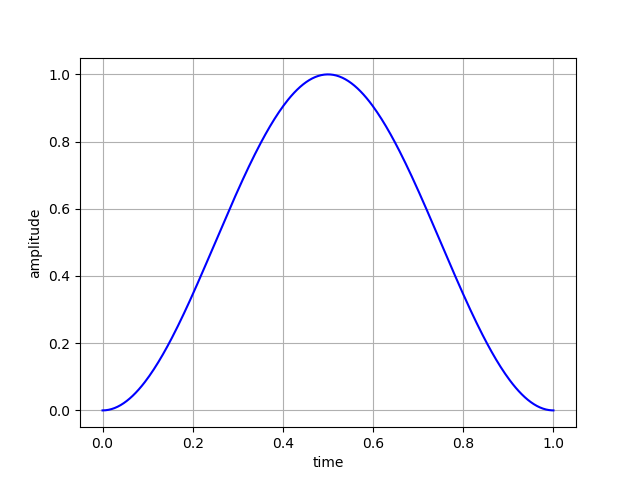
\includegraphics[width=\textwidth]{Figures/hanning300}
\caption{The Hanning window.}
\label{fig:Hanning}
\end{figure}

Figure~\ref{fig:Sample Input} shows a sample input data sequence,
for simplicity just a sine function.
%
\begin{figure}[tb]
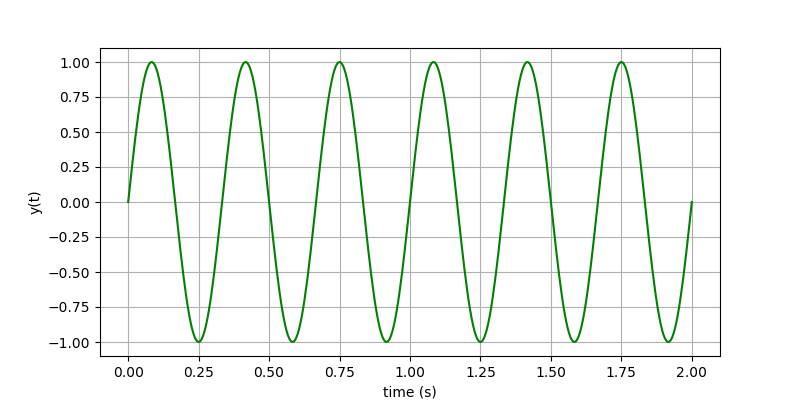
\includegraphics[width=\textwidth]{Figures/input}
\caption{Sample input data.}
\label{fig:Sample Input}
\end{figure}
%
Each data segment will then be captured by overlapping and window tapering
such that the sum of all data segments is equal to the original,
except at the ends where the window is still present.
An easy way to accomplish this is to use the Hanning window with 50\% overlap,
as showed in Figure~\ref{fig:Overlapping Hanning}.
%
\begin{figure}[!tb]
\center
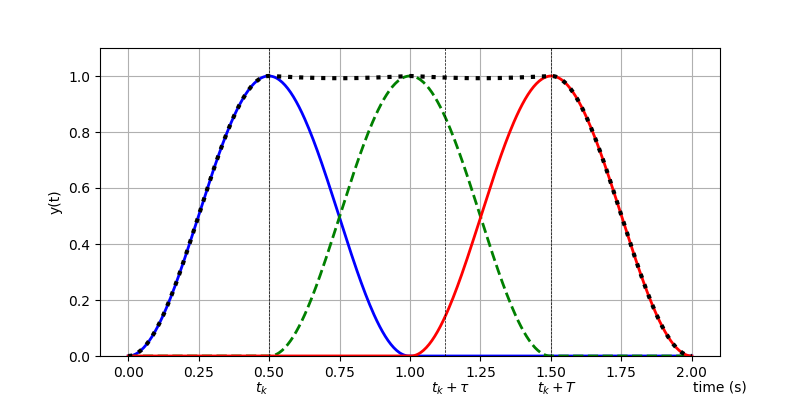
\includegraphics[width=\textwidth]{Figures/movingHenning}
\caption{Three Hanning windows with 50\% overlap.}
\label{fig:Overlapping Hanning}
\end{figure}
%
The additional dashed black line represents the superposition of the overlapped
windows, which results in unity except for at the ends of the sequences where
the window is still present.
Figure~\ref{fig:Tapered data} shows the tapered data segments for three
Hanning windows, which are obtained by multiplying the window function
with the input data-sequence.
The product is zero-valued outside the interval.
All that is left is the part where they coincide,
the ``view through the window''.
This input data isolation (tapering) is the main purpose of window functions.
%
\begin{figure}[tb]
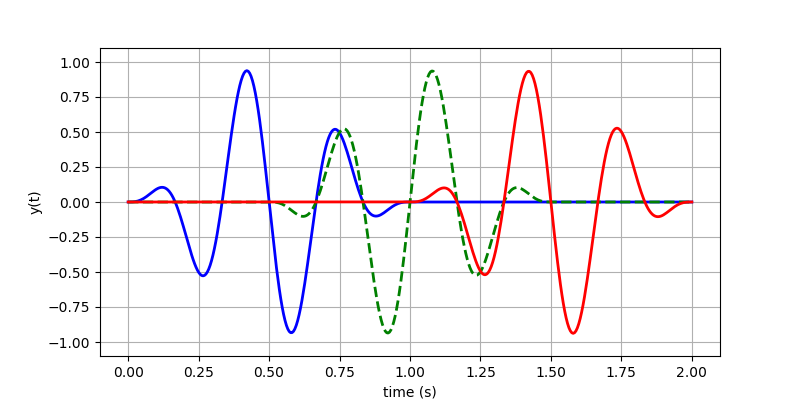
\includegraphics[width=\textwidth]{Figures/tapered}
\caption{Tapered windows.}
\label{fig:Tapered data}
\end{figure}

It is convenient to perform the windowing and overlapping between segments in
such a way that the windowed data segments are defined in terms of the
absolute time, i.e.,
%
\begin{equation}
\label{eq:wind}
y_k(t) \;=\:
\begin{cases}
y(t)\,\omega(t-t_k) & t\subset\left[t_k,t_k+T\right] \\
      0             & t\not\subset\left[t_k,t_k+T\right]
\end{cases}
\end{equation}
%
For each of these tapered windows, a Fast Fourier Transform (FFT) into the
frequency domain, and an inverse FFT back to time domain will be applied.
After assembling, the `tapered system response'
(see Figure~\ref{fig:Tapered system response}) will be obtained.
As mentioned above, at the ends the window lobes are still active.
%
\begin{figure}[tb]
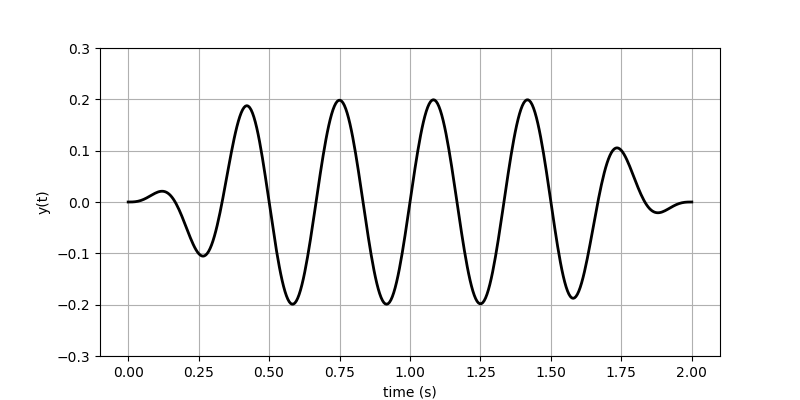
\includegraphics[width=\textwidth]{Figures/response}
\caption{Tapered system response}
\label{fig:Tapered system response}
\end{figure}
%
The systems response in Figure~\ref{fig:Tapered system response}
is based on an undamped system.
The transfer function reduces the amplitude, and there is no phase shift
because the system is undamped and not in resonance.

The window size $N_w$ represents the number of samples and herefrom the
duration $T_w$ (see \eqnref{eq:wtime}).
It depends on the fundamental frequency, intensity and change. In general:
{\it The lower the frequency, the bigger the window size should be.}
The default behaviour in Fedem is to not use windowing and to treat the entire
time series of the simulation in one go.

%%%%%%%%%%%%%%%%%%%%%%%%%%%%%%%%%%%%%%%%%%%%%%%%%%%%%%%%%%%%%%%%%%%%%%%%%%%%%%%%
\subsection{Fast fourier transformation (FFT)}
\label{subs:Fast fourier transformation}

A Fourier transform takes a signal in the time domain and
switches it into the frequency domain, e.g., it transforms a time series
$f(t)$ of $N$ equally- or uniformly spaced points in time $t_n=n\Delta t$,
$n=0,\ldots,N-1$, from the discrete time (or spatial) domain
to the discrete frequency domain.
The inverse Fourier transform does the inverse transformation from the
frequency domain back to the time (or spatial) domain.

The discrete Fourier transform (DFT) is defined given by
%
\begin{equation}
\label{eq:dft_sum0}
X_k \;=\; \sum_{n=0}^{N-1} x_n e^{-{i2\pi kn}/N}
\end{equation}
%
where $x_n$ are the values of a signal at equally spaced times $n=0,\ldots,N-1$.
The output $X_k$ is a complex number which encodes the amplitude and phase of a
sinusoidal wave with frequency $k/N$ cycles per time unit\footnote{This comes
from Euler's formula:
$\exp(\frac{i2\pi kn}{N}) = \cos(\frac{2\pi kn}{N}) + i\sin(\frac{2\pi kn}{N})
$.}.
The effect of computing $X_k$ is to find the coefficients of a signal
approximation by a linear combination of such waves.
Since each wave has a whole number of cycles per $N$ time units,
the approximation will be periodic with period $N$.
This approximation is given by the inverse Fourier transform
%
\begin{equation}
\label{eq:dft_sum1}
x_n \;=\; \frac{1}{N} \sum_{k=0}^{N-1} X_k e^{i2\pi kn}/N
\end{equation}
%
with
%
\vskip\baselineskip
\begin{namelist}{$n/N$}
\item[$N$] number of time samples
\item[$n$] current sample ($0,\ldots,N-1$)
\item[$x_n$] value of the signal at time $t_n$
\item[$k$] current frequency from 0 Hz up to $N-1$ Hz
\item[$X_k$] amount of frequency $k$ in the signal (amplitude and phase)
\item[$1/N$] normalization factor
\item[$n/N$] percent of "going through" time, $2\pi k$ speed in radians/sec
\end{namelist}
%
\vskip0.5\baselineskip
The DFT can be efficiently computed by the Fast Fourier Transform (FFT) algorithm.

\subsubsection{Units and spacing}

Let $\Delta t$ denote the spacing between points in time
and $N$ be the number of points/time samples.
The spacing $\Delta f$ of the points in frequency is the $1/(N\Delta t)$.
The quantity $1/\Delta t$ is called the sampling frequency $f_s$,
which should be at least twice of the highest frequency that is present in the
underlying continuous signal.

\subsubsection{Nyquist frequency, aliasing, mirroring}

When all frequencies present in the underlying continuous signal are below the
Nyquist frequency $f_q=\frac{1}{2\Delta t}$, then the discretely sampled time
series contains all of the information in the original continuous signal.
This is known as the sampling theorem and is a remarkable fact.

If a frequency exceeds the Nyquist frequency, the power from that frequency is
still transferred to the FFT, but it gets mapped to a bin in the result as if it
had been wrapped around. This phenomena is termed aliasing.
One can think of the resulting spectrum as being a circular buffer, representing
signal at each frequency modulo the maximum frequency of $\frac{1}{\Delta t}$.
A frequency of $\frac{1}{2\Delta t}$ would map to the middle bin,
also frequencies of $\frac{3}{2\Delta t}$, $\frac{5}{2\Delta t}$ and so on.

\subsubsection{Amplitude and phase}

Each number in the result of FFT is a complex number, an encoding of both the
amplitude and phase shift of each frequency component.
For example, if a 200 Hz component is present, the magnitude of the result at
200 Hz (as given by the absolute value of complex numbers) gives the power
density at that frequency.
For recovering the original signal, the phase of the component is also relevant.
Even though the power density at a certain frequency $f$ is the same for a
$\sin(2\pi ft)$, a $\cos(2\pi ft)$, or a $\sin(2\pi ft + \phi_0)$,
the phase is different in each of these cases.

The absolute height of an FFT is sometimes confusing.
The FFT reflects the total energy of the signal,
including the positive and negative frequencies.
Only the positive frequencies are from interest and therefore for
getting the amplitudes of the input, the FFT must be multiplied by 2.

\subsubsection{Efficiency}

The FFT algorithm is a fast implementation of the Discrete Fourier Transform
(DFT), which is most efficient when the number of elements $N$ in $t$ and $f$
is an even power of 2.
The worst efficiency will occur if $N$ is a prime number,
the efficiency of the FFT decreases to the efficiency of the DFT itself.
A DFT requires $O(N^2)$ steps, a FFT requires $O(N\log(N))$ steps.

%%%%%%%%%%%%%%%%%%%%%%%%%%%%%%%%%%%%%%%%%%%%%%%%%%%%%%%%%%%%%%%%%%%%%%%%%%%%%%%%
\subsection{Modal damping}
\label{subs:Modal Damping}

Finding proper specification for the structural damping is one of the most
challenging input tasks, because verification is possible only by performing
a response analysis in the time domine.
One way to specify the damping is by means of modal damping,
where the frequency-dependent damping ratio as the percentage of the critical
damping is specified for each mode.
This will then result in a diagonal damping matrix associated with the modes.

The modal damping ratio can be calculated via
%
\begin{equation}
\label{eq:modal_damping}
\zeta_i \;=\; \frac{c_i}{c_{{\rm cr},i}}
\end{equation}
%
with the critical damping $c_{{\rm cr},i}=2m_i\omega_i$
and $\omega_i^2=\frac{k_i}{m_i}$.
The important characteristic in modal damping reflects that the damping values
are calculated at natural frequencies and not at the excitation frequencies.
